\documentclass[a4paper]{article}

\usepackage[english]{babel}
\usepackage[utf8]{inputenc}
\usepackage{amsmath}
\usepackage{graphicx}
\usepackage[breaklinks]{hyperref}
\usepackage{caption}
\usepackage[round]{natbib}
\bibliographystyle{plainnat}


\title{
	Project 02 \\
	\bigskip
	\normalsize APSC 607 Fall 2017
}

\author{Seth Goodman}

\date{\today}


\begin{document}
\maketitle


%\begin{abstract}
%\end{abstract}

\section{Introduction}
\label{sec:introduction}


This project explored methods for calculating the integral roots of functions. Each functions was  examined in the range between zero and two, using the Composite Trapezoidal Rule, Composite Midpoint Rule, Composite Simpson’s Rule, as well as an adaptive implementation of the Composite Simpson’s Rule. The behavior and characteristics of these methods are reviewed by examining the effectiveness of the resulting value for the integral given a range of values for N. 

All computations were performed using MATLAB using the code accompanying this report (in a zip file). The following \textit{Methods} section will present the methods used in MATLAB to explore functions, as well as the outputs and results. The \textit{Results} section of this report contains the outputs for each function along with related observations and discussion. All figures and tables found in this report are available in the output subdirectory of the accompanying zip file. Additionally, all code and figures found in the zip file can be accessed via GitHub\footnote{\url{https://github.com/sgoodm/apsc607/tree/master/project_02}}.



\newpage
\section{Methods}
\label{sec:methods}

Equations \ref{eq:fa} and \ref{eq:fb} define the two function, hereafter referred to as Function \textbf{A} and \textbf{B}, respectively, which are examined in this project. Three different composite numerical integration approaches - Trapezoidal, Midpoint, and Simpson's - will be tested to examine the effectiveness of each method. A fourth adaptive approach based on Simpson's Rule will also be tested for comparison. Integration will be restricted to between zero and two for testing, but integration over an expanded range and the potential utility of adaptive approaches in such a scenario will be discussed in the \textit{Results} section.

\begin{equation}
f(x) = e^{2x} * sin(3x)
\label{eq:fa}
\end{equation}

\begin{equation}
f(x) = \frac{1}{x+4}
\label{eq:fb}
\end{equation}


To establish a baseline, the true value for the integral of each function is first calculated using built in MATLAB tools. The integral is calculated both using the symbolic toolkit function \textbf{int} as well as the numerical function \textbf{integral}. The resulting values can be seen in Table \ref{true_values}.


\bgroup
\def\arraystretch{1.5}
\begin{center}
	\centering
	\begin{tabular}{l|r|r}
	\textbf{Function} & \textbf{Symbolic} & \textbf{Numeric} \\
	\hline
	A & -14.2139771298625 & -14.2139771298625\\
	B & 0.405465108108164 & 0.405465108108164
	\end{tabular}
	\captionof{table}{True values of integrals between zero and two}
	\label{true_values}
\end{center}
\egroup

The true value for Functions A and B will be compared to the results of integration using the Trapezoidal, Midpoint, and Simpson's Rules for a range of subintervals defined as \textbf{n}. The range of \textbf{n} will vary with each function and rule tested, in order to achieve accuracy within a tolerance of $1e^{-8}$.

The value of \textbf{n} required to reach the specified tolerance is dependent on the function itself as well as the error term associated with each rule. The error terms for the Trapezoidal, Midpoint, and Simpson's Rules are defined in Equation \ref{trap_err}, \ref{mid_err}, and \ref{sim_err} respective \citep{burden2010}. As the Trapezoidal and Midpoint Rules have second order error terms, it is expected that they will require a greater value of \textbf{n} to produce results comparable to Simpson's Rule, which has a fourth order error term.

\begin{equation}
\frac{b-a}{6}h^2f^{''}(u)
\label{trap_err}
\end{equation}

\begin{equation}
\frac{b-a}{12}h^2f^{''}(u)
\label{mid_err}
\end{equation}

\begin{equation}
\frac{h^5}{90}f^{(4)}(\xi_j)
\label{sim_err}
\end{equation}

All values of \textbf{n} tested will be positive and even, as it is required for the Midpoint and Simpson's Rules. Although the Trapezoidal Rule can be performed using odd intervals, using only even intervals will provide sufficient sample points for analysis. In order to test \textbf{n} over a sufficient range for the Trapezoidal and Midpoint Rules, a binary expansion was used to generate values of \textbf{n} at which to sample the full range, rather than test at every possible step. Starting with two sub intervals ($n=2$), if every even sub interval value up to 100,000 was tested it would require 50,000 points. By incorporating a binary expansion based approach, a sample of only 20 different \textbf{n} values can generated which are capable of sufficiently demonstrating the behavior of the integration rules.

Due to the higher order error term, Simpson's Rule can reach the desired tolerance much quicker and a simple range of $2:2:nmax$ can be used. Finally, no \textbf{n} value needs to be specified for the adaptive approach because, as seen in Subsection \ref{method:adaptive}, this approach iteratively checks that a specified tolerance has been reached before producing an output rather than using a set \textbf{n} value.

The remainder of this section will introduce the three composite numerical integration approaches (Trapezoidal, Midpoint, and Simpson's) as well as an adaptive approach using Simpson's Rule.


\subsection{Composite Trapezoidal Rule}\label{method:trapezoidal}
TEXT

\begin{center}

	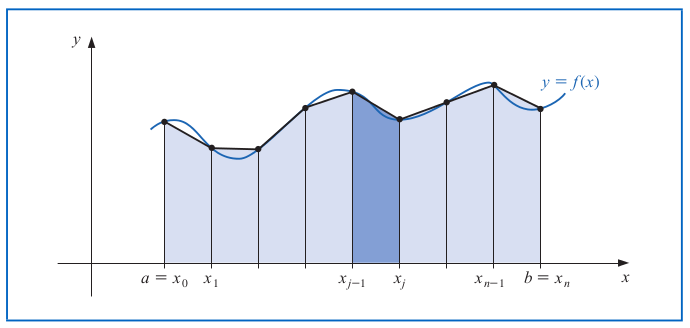
\includegraphics[width=1\textwidth]{../additional/trapezoidal_fig.png}
	\captionof{figure}{Trapezoidal Figure \citep{burden2010}}
	\label{trap_fig}
\end{center}


The Composite Trapezoidal Rule for $n$ intervals, as seen in Figure \ref{trap_fig}, can be defined by Equation \ref{trap_eq}, given $h=(b-a)/n$ and $x_j=a+jh$, for each $j=0,1,\dots,n$ \citep{burden2010}.

\begin{equation}
\int_{a}^b f(x) dx = \frac{h}{2} \Bigg[ f(a) + 2 \sum_{j=1}^{n-1} f(x_j) + f(b) \Bigg]
\label{trap_eq}
\end{equation}

Implementing this in a MATLAB function is extremely straightforward. The function accepts a function handle \textbf{f} defining $f(x)$, (e.g., $cos(x)$), the desired number of internval \textbf{n}, along with our bounds \textbf{rmin} and \textbf{rmax}. The value for \textbf{h} given \textbf{n} is calculated, as are the vectors \textbf{j} and \textbf{$x_j$}. Using these components and the summation function, the final integral for the input conditions can be calculated. The function then returns the integral value, along with the value of \textbf{h} used.

This function implementing the Trapezoidal Rule for integration (as well as subsequent Midpoint and Simpson's Rules) is called over a range of values for \textbf{n} using the \textbf{arrayfun} function in MATLAB. This function accepts another function, defining our integration rule, and a vector, and simply repeatedly calls the specified value while iterating over the values in the vector. The call to \textbf{arrayfun} then return a vector (or set of vectors in this case) containg the results from each call to the integration function.

 The resulting vector of integral values across varying \textbf{n} can compared with the true integral value generated earlier, to produce an error vector. The error vector is used to identify the value of \textbf{n} (and thus \textbf{h}) at which the integration rule produced results that were accurate within a desired tolerance.



\subsection{Composite Midpoint Rule}\label{method:midpoint}
TEXT

\begin{center}
	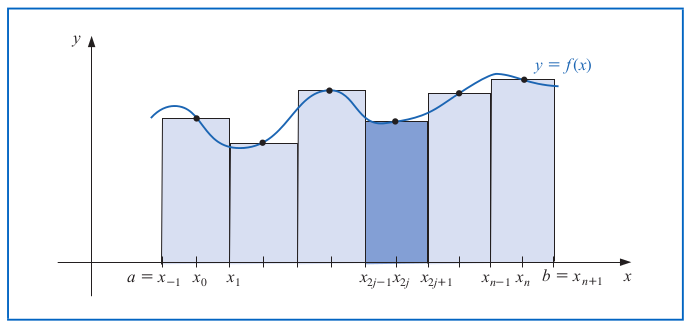
\includegraphics[width=1\textwidth]{../additional/midpoint_fig.png}
	\captionof{figure}{Midpoint Figure \citep{burden2010}}
	\label{mid_fig}
\end{center}

The Composite Midpoint Rule for $n+2$ intervals, as seen in Figure \ref{mid_fig}, can be defined by Equation \ref{mid_eq}, given $h=(b-a)/(n+2)$ and $x_j=a+(j+1)h$, for each $j=-1,0,\dots,n+1$ \citep{burden2010}.

\begin{equation}
\int_{a}^b f(x) dx = 2h \sum_{j=0}^{n/2}f(x_2j)
\label{mid_eq}
\end{equation}

\subsection{Composite Simpson's Rule}\label{method:simpsons}
TEXT

\begin{center}
	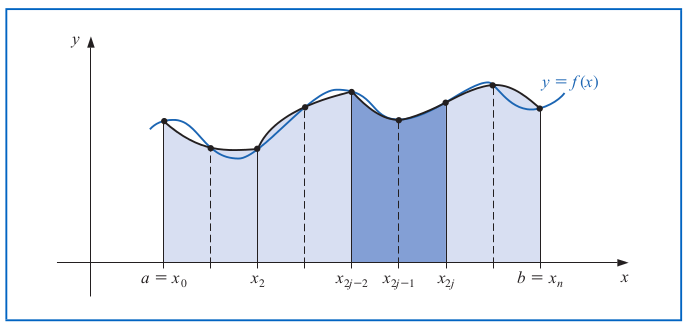
\includegraphics[width=1\textwidth]{../additional/simpsons_fig.png}
	\captionof{figure}{Simpson's Figure \citep{burden2010}}
	\label{sim_fig}
\end{center}

The Composite Simpson's Rule for $n$ intervals, as seen in Figure \ref{sim_fig}, can be defined by Equation \ref{sim_eq}, given $h=(b-a)/n$ and $x0_j=a+jh$, $x1_j=a+jh+h/2$, $x2_j=a+jh+h$,  for each $j=0,1,\dots,n-1$.
 
    
\begin{equation}
\int_{a}^b f(x) dx = \sum_{j=0}^{n-1} \Bigg[ \frac{h}{6} \big[ f(x0_j) + 4f(x1_j) + f(x2_j) \big] \Bigg]
\label{sim_eq}
\end{equation}



\subsection{Adaptive Simpson's Rule}\label{method:adaptive}
TEXT



\newpage
\section{Results}
\label{sec:results}

TEXT



\subsection{A}\label{results:a}

\begin{center}
	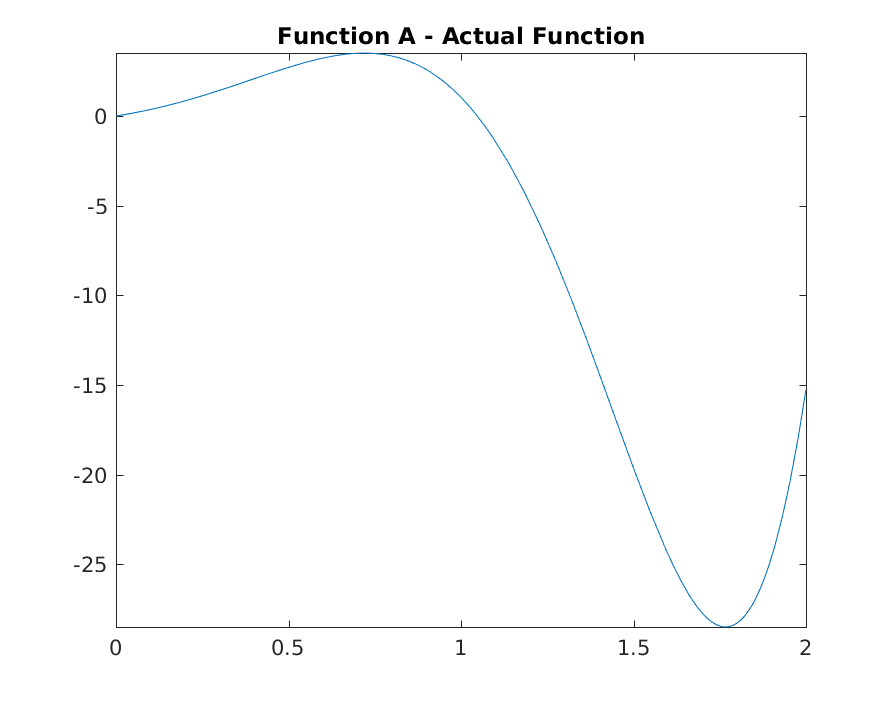
\includegraphics[width=1\textwidth]{../output/a_actual.png}
	\captionof{figure}{caption text a}
	\label{fig:a_act}
\end{center}

\begin{center}
	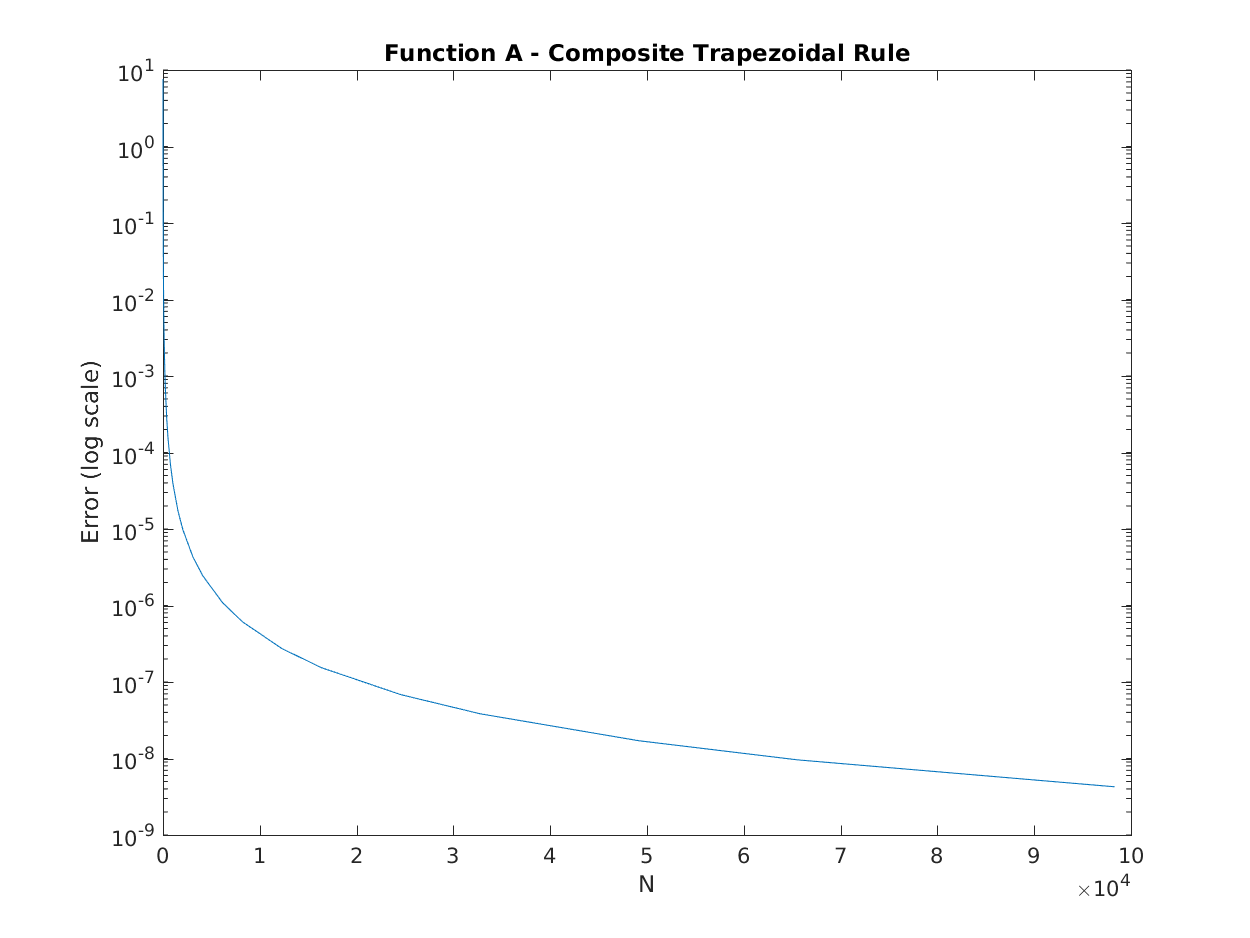
\includegraphics[width=1\textwidth]{../output/a_trapezoidal.png}
	\captionof{figure}{caption text a}
	\label{fig:a_trap}
\end{center}


\begin{center}
	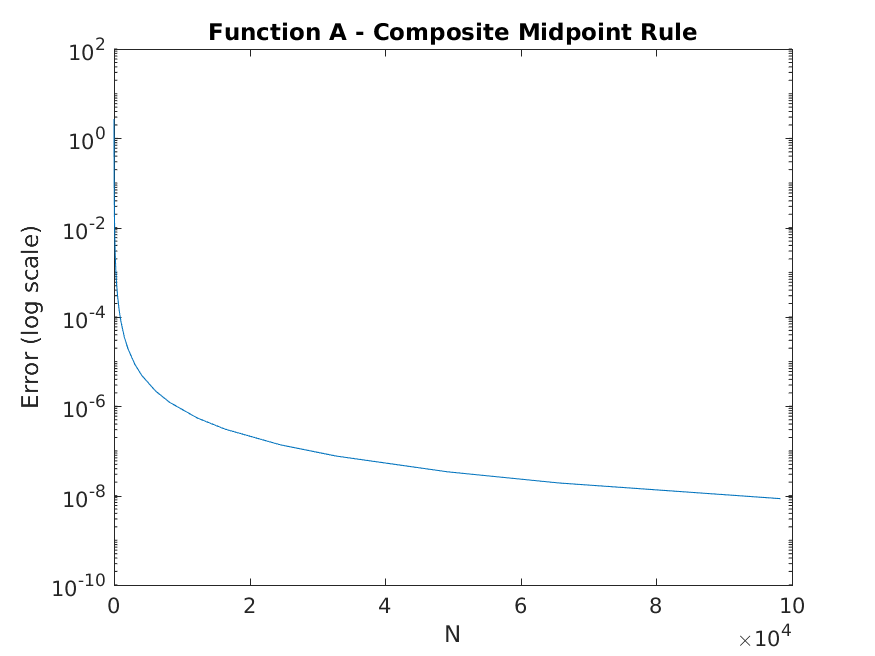
\includegraphics[width=1\textwidth]{../output/a_midpoint.png}
	\captionof{figure}{caption text a}
	\label{fig:a_mid}
\end{center}


\begin{center}
	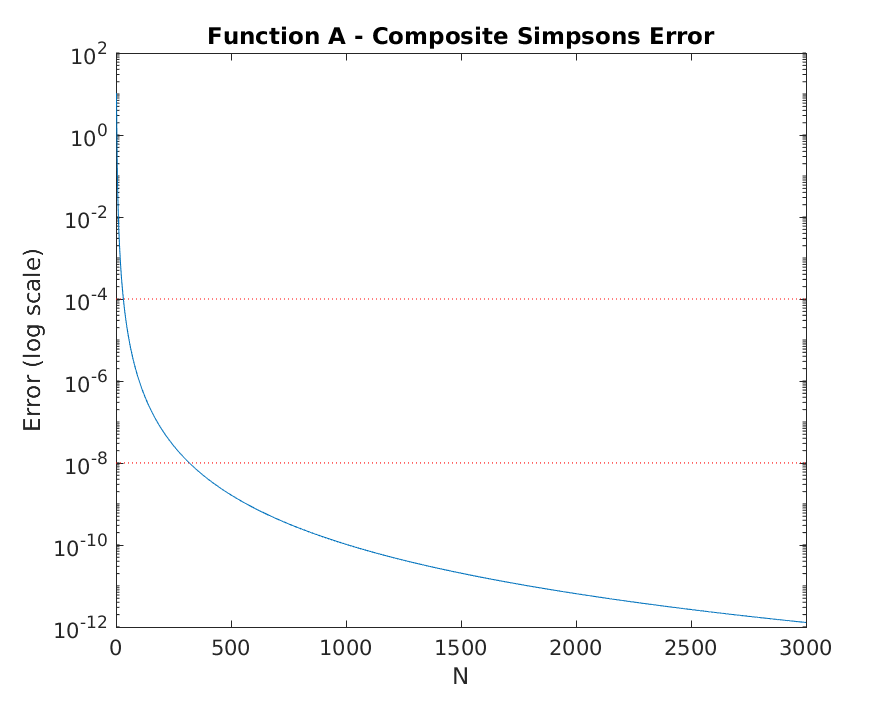
\includegraphics[width=1\textwidth]{../output/a_simpsons.png}
	\captionof{figure}{caption text a}
	\label{fig:a_sim}
\end{center}


\begin{center}
	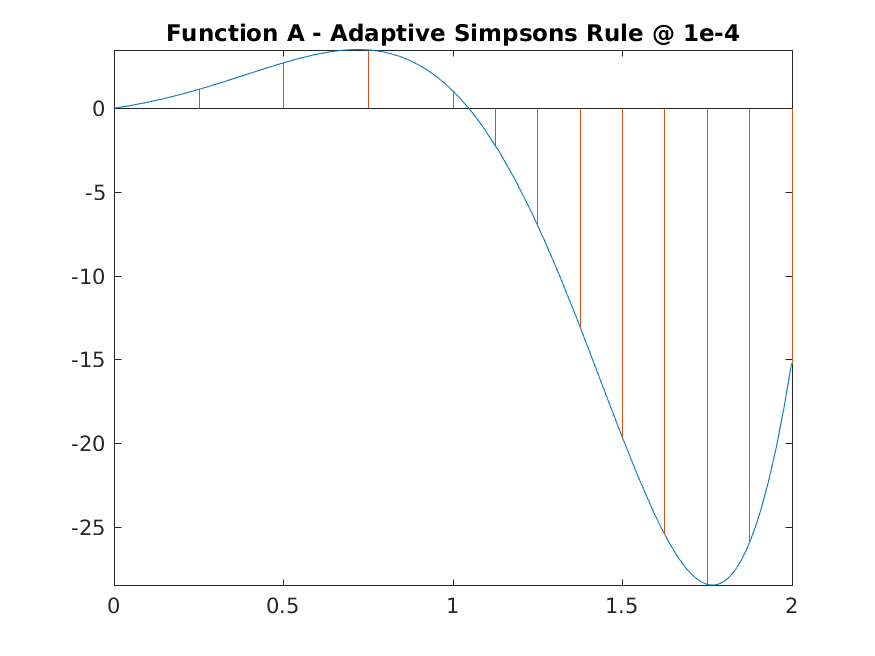
\includegraphics[width=1\textwidth]{../output/a_adaptive_simpsons_4.png}
	\captionof{figure}{caption text a}
	\label{fig:a_adap4}
\end{center}

\begin{center}
	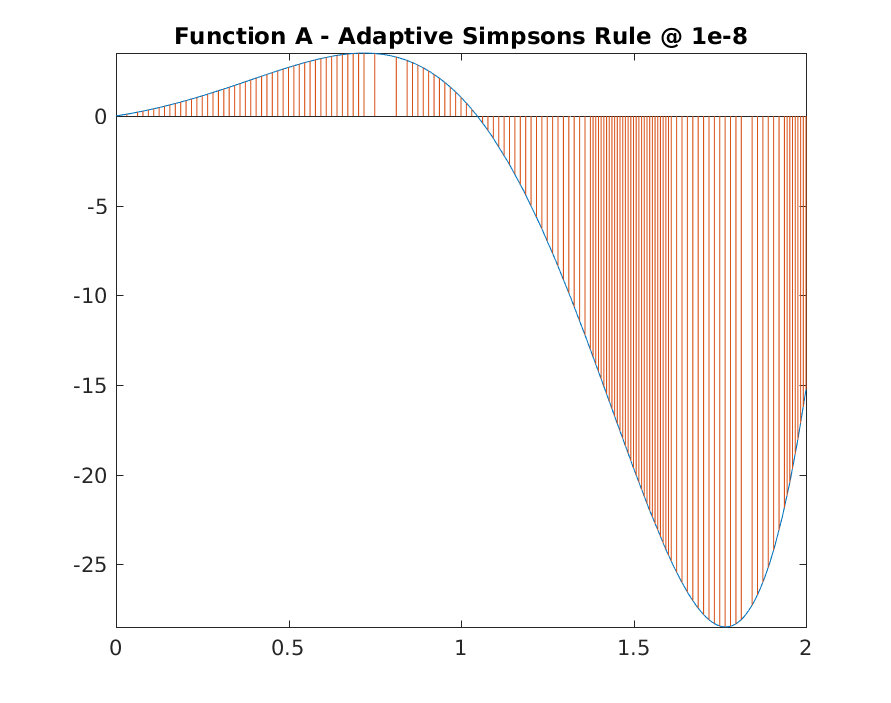
\includegraphics[width=1\textwidth]{../output/a_adaptive_simpsons_8.png}
	\captionof{figure}{caption text a}
	\label{fig:a_adap8}
\end{center}



\subsection{B}\label{results:b}

\begin{center}
	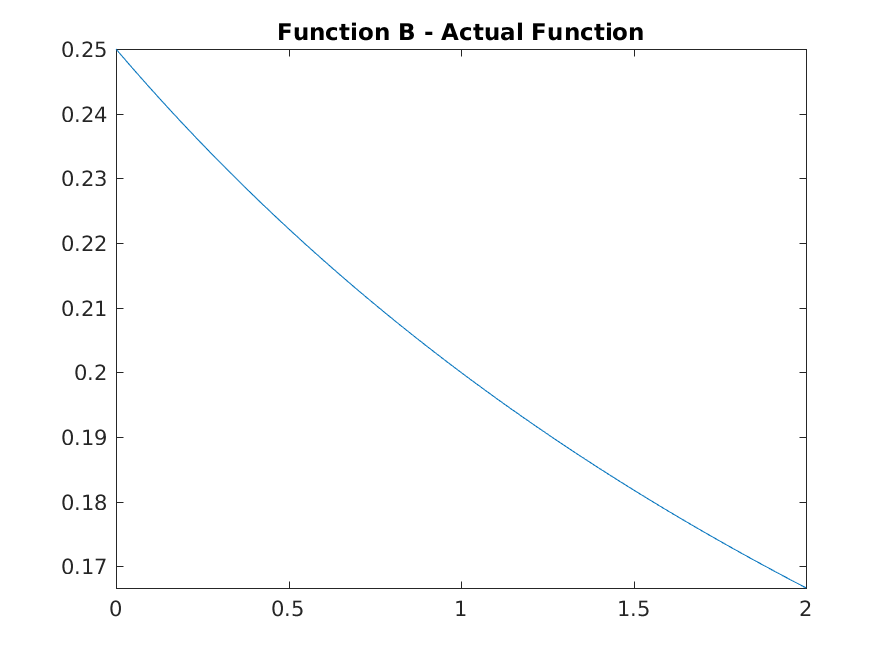
\includegraphics[width=1\textwidth]{../output/b_actual.png}
	\captionof{figure}{caption text a}
	\label{fig:b_act}
\end{center}

\begin{center}
	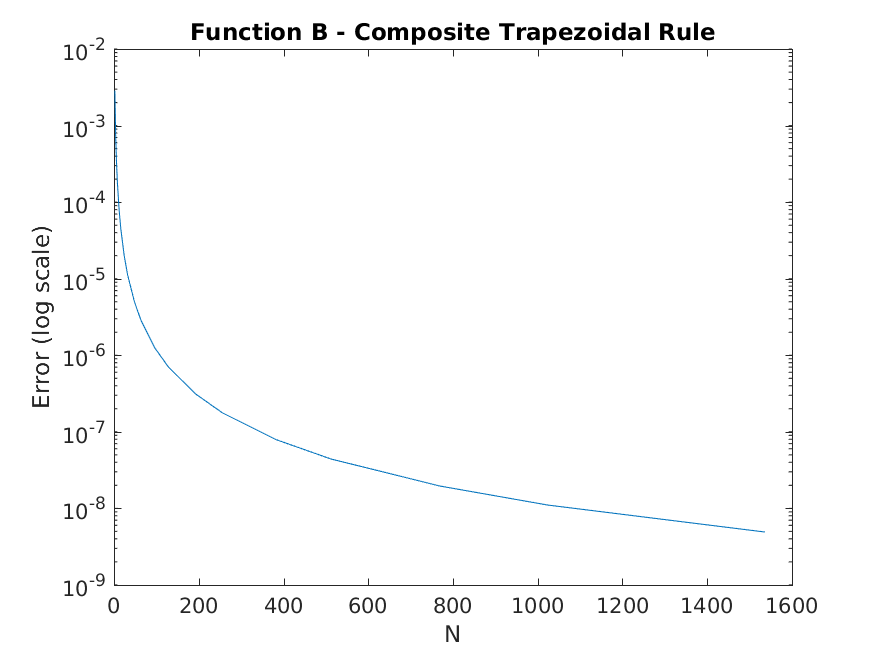
\includegraphics[width=1\textwidth]{../output/b_trapezoidal.png}
	\captionof{figure}{caption text a}
	\label{fig:b_trap}
\end{center}


\begin{center}
	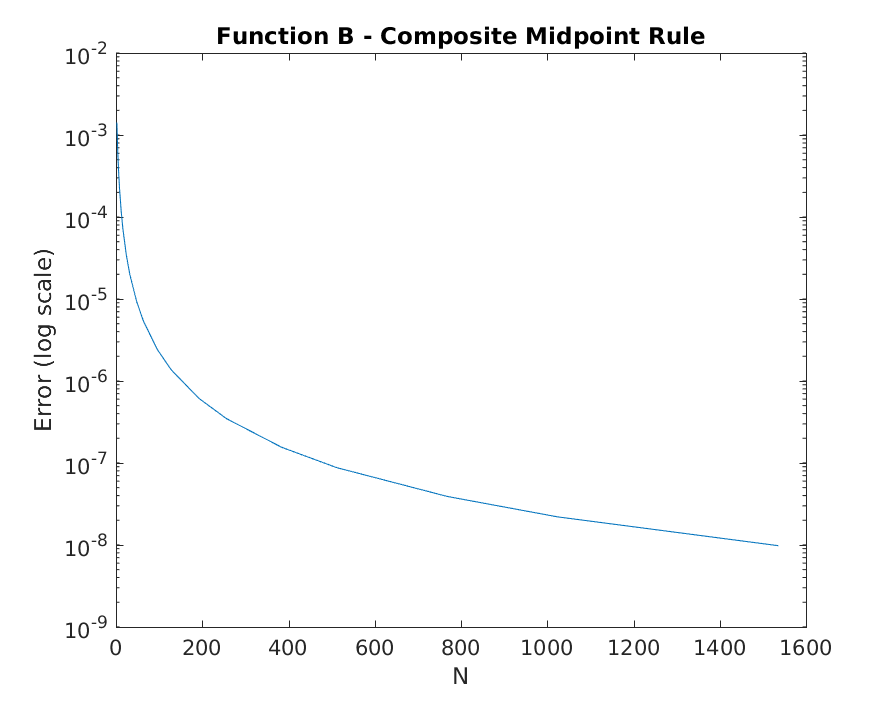
\includegraphics[width=1\textwidth]{../output/b_midpoint.png}
	\captionof{figure}{caption text a}
	\label{fig:b_mid}
\end{center}


\begin{center}
	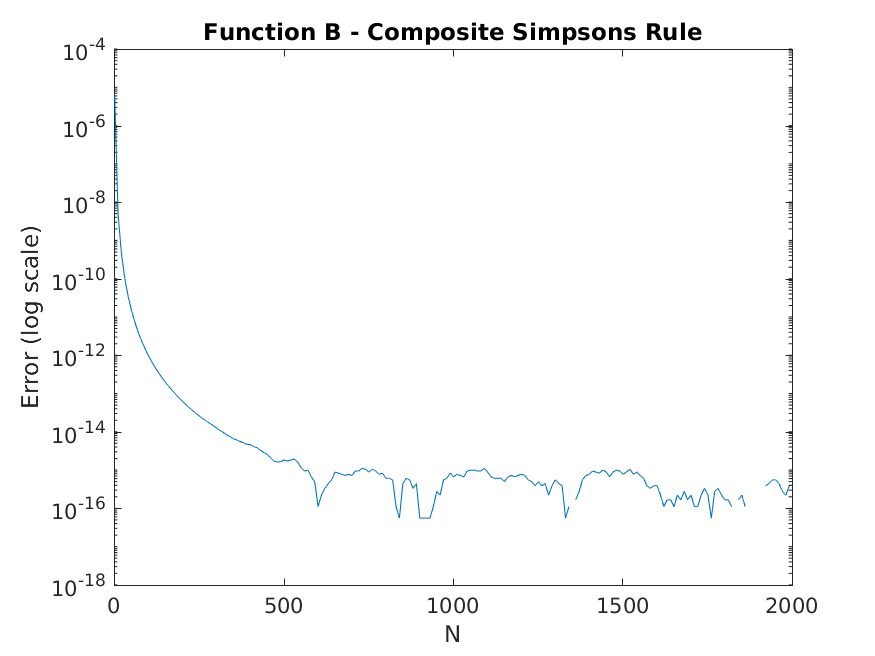
\includegraphics[width=1\textwidth]{../output/b_simpsons.png}
	\captionof{figure}{caption text a}
	\label{fig:b_sim}
\end{center}


\begin{center}
	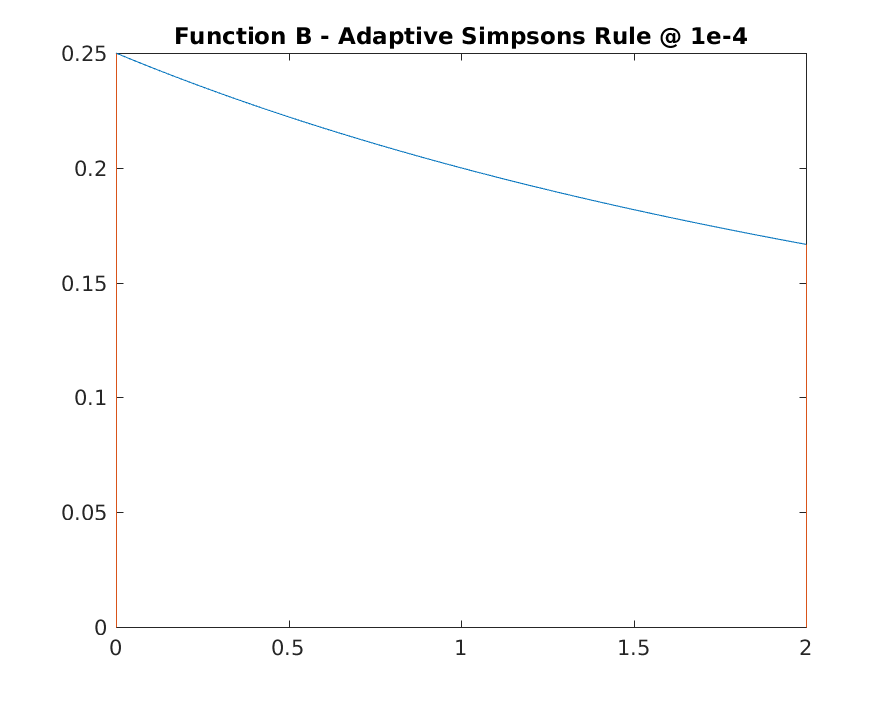
\includegraphics[width=1\textwidth]{../output/b_adaptive_simpsons_4.png}
	\captionof{figure}{caption text a}
	\label{fig:b_adap4}
\end{center}

\begin{center}
	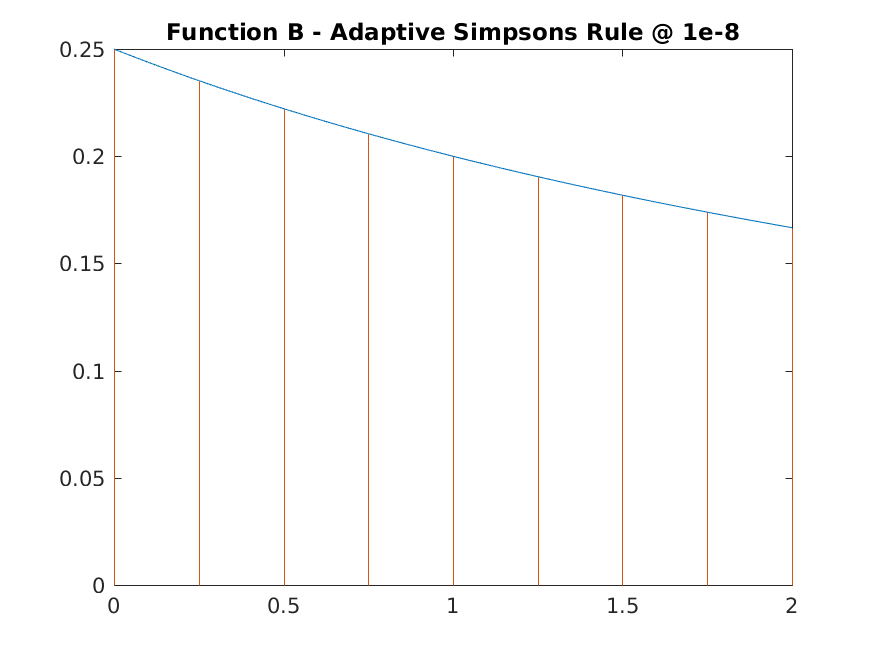
\includegraphics[width=1\textwidth]{../output/b_adaptive_simpsons_8.png}
	\captionof{figure}{caption text a}
	\label{fig:b_adap8}
\end{center}






\subsection{Expanded Range}\label{results:expanded}


\begin{center}
	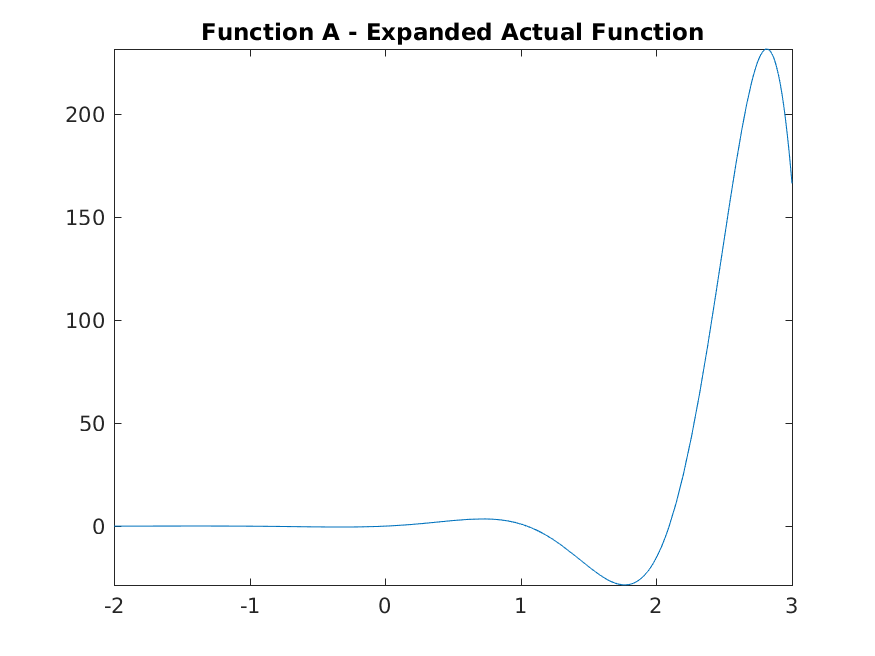
\includegraphics[width=1\textwidth]{../output/a_expanded_actual.png}
	\captionof{figure}{caption text a}
	\label{fig:a_ex}
\end{center}


\begin{center}
	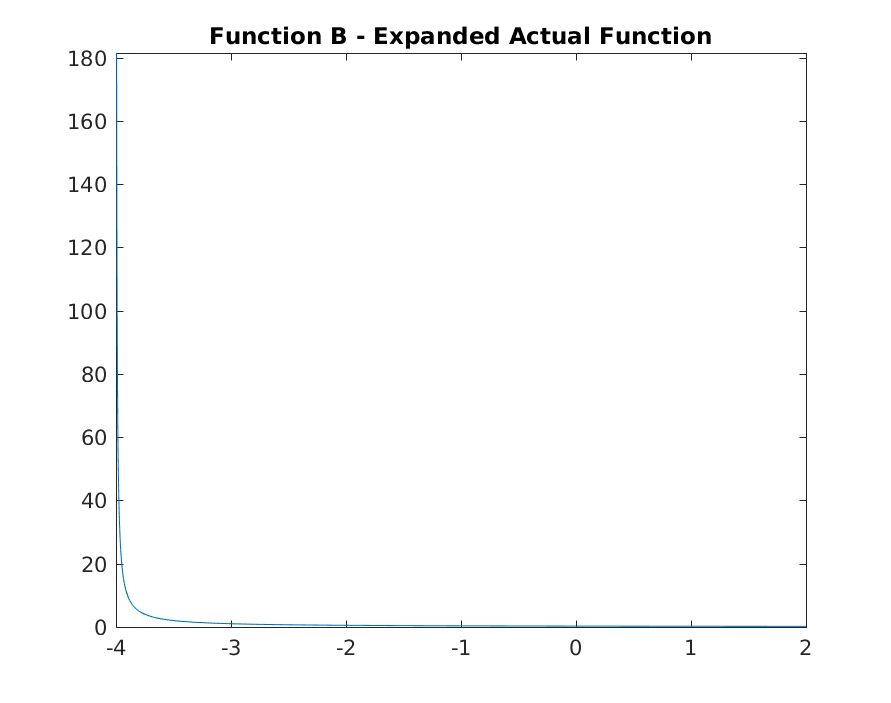
\includegraphics[width=1\textwidth]{../output/b_expanded_actual.png}
	\captionof{figure}{caption text a}
	\label{fig:b_ex}
\end{center}








Something about minimum error in footnote\footnote{See following link on MATLAB precision limitions (general limitations of floating point representations apply) https://www.mathworks.com/help/fixedpoint/ug/limitations-on-precision.html}.




\newpage

\bibliography{report}


\end{document}
